% Options for packages loaded elsewhere
\PassOptionsToPackage{unicode}{hyperref}
\PassOptionsToPackage{hyphens}{url}
\PassOptionsToPackage{dvipsnames,svgnames,x11names}{xcolor}
%
\documentclass[
  letterpaper,
  DIV=11,
  numbers=noendperiod]{scrartcl}

\usepackage{amsmath,amssymb}
\usepackage{iftex}
\ifPDFTeX
  \usepackage[T1]{fontenc}
  \usepackage[utf8]{inputenc}
  \usepackage{textcomp} % provide euro and other symbols
\else % if luatex or xetex
  \usepackage{unicode-math}
  \defaultfontfeatures{Scale=MatchLowercase}
  \defaultfontfeatures[\rmfamily]{Ligatures=TeX,Scale=1}
\fi
\usepackage{lmodern}
\ifPDFTeX\else  
    % xetex/luatex font selection
\fi
% Use upquote if available, for straight quotes in verbatim environments
\IfFileExists{upquote.sty}{\usepackage{upquote}}{}
\IfFileExists{microtype.sty}{% use microtype if available
  \usepackage[]{microtype}
  \UseMicrotypeSet[protrusion]{basicmath} % disable protrusion for tt fonts
}{}
\makeatletter
\@ifundefined{KOMAClassName}{% if non-KOMA class
  \IfFileExists{parskip.sty}{%
    \usepackage{parskip}
  }{% else
    \setlength{\parindent}{0pt}
    \setlength{\parskip}{6pt plus 2pt minus 1pt}}
}{% if KOMA class
  \KOMAoptions{parskip=half}}
\makeatother
\usepackage{xcolor}
\setlength{\emergencystretch}{3em} % prevent overfull lines
\setcounter{secnumdepth}{-\maxdimen} % remove section numbering
% Make \paragraph and \subparagraph free-standing
\ifx\paragraph\undefined\else
  \let\oldparagraph\paragraph
  \renewcommand{\paragraph}[1]{\oldparagraph{#1}\mbox{}}
\fi
\ifx\subparagraph\undefined\else
  \let\oldsubparagraph\subparagraph
  \renewcommand{\subparagraph}[1]{\oldsubparagraph{#1}\mbox{}}
\fi

\usepackage{color}
\usepackage{fancyvrb}
\newcommand{\VerbBar}{|}
\newcommand{\VERB}{\Verb[commandchars=\\\{\}]}
\DefineVerbatimEnvironment{Highlighting}{Verbatim}{commandchars=\\\{\}}
% Add ',fontsize=\small' for more characters per line
\usepackage{framed}
\definecolor{shadecolor}{RGB}{241,243,245}
\newenvironment{Shaded}{\begin{snugshade}}{\end{snugshade}}
\newcommand{\AlertTok}[1]{\textcolor[rgb]{0.68,0.00,0.00}{#1}}
\newcommand{\AnnotationTok}[1]{\textcolor[rgb]{0.37,0.37,0.37}{#1}}
\newcommand{\AttributeTok}[1]{\textcolor[rgb]{0.40,0.45,0.13}{#1}}
\newcommand{\BaseNTok}[1]{\textcolor[rgb]{0.68,0.00,0.00}{#1}}
\newcommand{\BuiltInTok}[1]{\textcolor[rgb]{0.00,0.23,0.31}{#1}}
\newcommand{\CharTok}[1]{\textcolor[rgb]{0.13,0.47,0.30}{#1}}
\newcommand{\CommentTok}[1]{\textcolor[rgb]{0.37,0.37,0.37}{#1}}
\newcommand{\CommentVarTok}[1]{\textcolor[rgb]{0.37,0.37,0.37}{\textit{#1}}}
\newcommand{\ConstantTok}[1]{\textcolor[rgb]{0.56,0.35,0.01}{#1}}
\newcommand{\ControlFlowTok}[1]{\textcolor[rgb]{0.00,0.23,0.31}{#1}}
\newcommand{\DataTypeTok}[1]{\textcolor[rgb]{0.68,0.00,0.00}{#1}}
\newcommand{\DecValTok}[1]{\textcolor[rgb]{0.68,0.00,0.00}{#1}}
\newcommand{\DocumentationTok}[1]{\textcolor[rgb]{0.37,0.37,0.37}{\textit{#1}}}
\newcommand{\ErrorTok}[1]{\textcolor[rgb]{0.68,0.00,0.00}{#1}}
\newcommand{\ExtensionTok}[1]{\textcolor[rgb]{0.00,0.23,0.31}{#1}}
\newcommand{\FloatTok}[1]{\textcolor[rgb]{0.68,0.00,0.00}{#1}}
\newcommand{\FunctionTok}[1]{\textcolor[rgb]{0.28,0.35,0.67}{#1}}
\newcommand{\ImportTok}[1]{\textcolor[rgb]{0.00,0.46,0.62}{#1}}
\newcommand{\InformationTok}[1]{\textcolor[rgb]{0.37,0.37,0.37}{#1}}
\newcommand{\KeywordTok}[1]{\textcolor[rgb]{0.00,0.23,0.31}{#1}}
\newcommand{\NormalTok}[1]{\textcolor[rgb]{0.00,0.23,0.31}{#1}}
\newcommand{\OperatorTok}[1]{\textcolor[rgb]{0.37,0.37,0.37}{#1}}
\newcommand{\OtherTok}[1]{\textcolor[rgb]{0.00,0.23,0.31}{#1}}
\newcommand{\PreprocessorTok}[1]{\textcolor[rgb]{0.68,0.00,0.00}{#1}}
\newcommand{\RegionMarkerTok}[1]{\textcolor[rgb]{0.00,0.23,0.31}{#1}}
\newcommand{\SpecialCharTok}[1]{\textcolor[rgb]{0.37,0.37,0.37}{#1}}
\newcommand{\SpecialStringTok}[1]{\textcolor[rgb]{0.13,0.47,0.30}{#1}}
\newcommand{\StringTok}[1]{\textcolor[rgb]{0.13,0.47,0.30}{#1}}
\newcommand{\VariableTok}[1]{\textcolor[rgb]{0.07,0.07,0.07}{#1}}
\newcommand{\VerbatimStringTok}[1]{\textcolor[rgb]{0.13,0.47,0.30}{#1}}
\newcommand{\WarningTok}[1]{\textcolor[rgb]{0.37,0.37,0.37}{\textit{#1}}}

\providecommand{\tightlist}{%
  \setlength{\itemsep}{0pt}\setlength{\parskip}{0pt}}\usepackage{longtable,booktabs,array}
\usepackage{calc} % for calculating minipage widths
% Correct order of tables after \paragraph or \subparagraph
\usepackage{etoolbox}
\makeatletter
\patchcmd\longtable{\par}{\if@noskipsec\mbox{}\fi\par}{}{}
\makeatother
% Allow footnotes in longtable head/foot
\IfFileExists{footnotehyper.sty}{\usepackage{footnotehyper}}{\usepackage{footnote}}
\makesavenoteenv{longtable}
\usepackage{graphicx}
\makeatletter
\def\maxwidth{\ifdim\Gin@nat@width>\linewidth\linewidth\else\Gin@nat@width\fi}
\def\maxheight{\ifdim\Gin@nat@height>\textheight\textheight\else\Gin@nat@height\fi}
\makeatother
% Scale images if necessary, so that they will not overflow the page
% margins by default, and it is still possible to overwrite the defaults
% using explicit options in \includegraphics[width, height, ...]{}
\setkeys{Gin}{width=\maxwidth,height=\maxheight,keepaspectratio}
% Set default figure placement to htbp
\makeatletter
\def\fps@figure{htbp}
\makeatother

\KOMAoption{captions}{tableheading}
\makeatletter
\makeatother
\makeatletter
\makeatother
\makeatletter
\@ifpackageloaded{caption}{}{\usepackage{caption}}
\AtBeginDocument{%
\ifdefined\contentsname
  \renewcommand*\contentsname{Table of contents}
\else
  \newcommand\contentsname{Table of contents}
\fi
\ifdefined\listfigurename
  \renewcommand*\listfigurename{List of Figures}
\else
  \newcommand\listfigurename{List of Figures}
\fi
\ifdefined\listtablename
  \renewcommand*\listtablename{List of Tables}
\else
  \newcommand\listtablename{List of Tables}
\fi
\ifdefined\figurename
  \renewcommand*\figurename{Figure}
\else
  \newcommand\figurename{Figure}
\fi
\ifdefined\tablename
  \renewcommand*\tablename{Table}
\else
  \newcommand\tablename{Table}
\fi
}
\@ifpackageloaded{float}{}{\usepackage{float}}
\floatstyle{ruled}
\@ifundefined{c@chapter}{\newfloat{codelisting}{h}{lop}}{\newfloat{codelisting}{h}{lop}[chapter]}
\floatname{codelisting}{Listing}
\newcommand*\listoflistings{\listof{codelisting}{List of Listings}}
\makeatother
\makeatletter
\@ifpackageloaded{caption}{}{\usepackage{caption}}
\@ifpackageloaded{subcaption}{}{\usepackage{subcaption}}
\makeatother
\makeatletter
\@ifpackageloaded{tcolorbox}{}{\usepackage[skins,breakable]{tcolorbox}}
\makeatother
\makeatletter
\@ifundefined{shadecolor}{\definecolor{shadecolor}{rgb}{.97, .97, .97}}
\makeatother
\makeatletter
\makeatother
\makeatletter
\makeatother
\ifLuaTeX
  \usepackage{selnolig}  % disable illegal ligatures
\fi
\IfFileExists{bookmark.sty}{\usepackage{bookmark}}{\usepackage{hyperref}}
\IfFileExists{xurl.sty}{\usepackage{xurl}}{} % add URL line breaks if available
\urlstyle{same} % disable monospaced font for URLs
\hypersetup{
  pdftitle={Analysis of variance},
  colorlinks=true,
  linkcolor={blue},
  filecolor={Maroon},
  citecolor={Blue},
  urlcolor={Blue},
  pdfcreator={LaTeX via pandoc}}

\title{Analysis of variance}
\author{}
\date{}

\begin{document}
\maketitle
\ifdefined\Shaded\renewenvironment{Shaded}{\begin{tcolorbox}[boxrule=0pt, breakable, frame hidden, sharp corners, interior hidden, enhanced, borderline west={3pt}{0pt}{shadecolor}]}{\end{tcolorbox}}\fi

\hypertarget{packages}{%
\subsection{Packages}\label{packages}}

\begin{Shaded}
\begin{Highlighting}[]
\FunctionTok{library}\NormalTok{(tidyverse)}
\end{Highlighting}
\end{Shaded}

\begin{verbatim}
-- Attaching core tidyverse packages ------------------------ tidyverse 2.0.0 --
v dplyr     1.1.2     v readr     2.1.4
v forcats   0.5.0     v stringr   1.5.0
v ggplot2   3.4.2     v tibble    3.2.1
v lubridate 1.9.2     v tidyr     1.3.0
v purrr     1.0.1     
-- Conflicts ------------------------------------------ tidyverse_conflicts() --
x dplyr::filter() masks stats::filter()
x dplyr::lag()    masks stats::lag()
i Use the conflicted package (<http://conflicted.r-lib.org/>) to force all conflicts to become errors
\end{verbatim}

\begin{Shaded}
\begin{Highlighting}[]
\FunctionTok{library}\NormalTok{(smmr)}
\FunctionTok{library}\NormalTok{(PMCMRplus)}
\end{Highlighting}
\end{Shaded}

\hypertarget{jumping-rats}{%
\subsection{Jumping rats}\label{jumping-rats}}

\begin{itemize}
\tightlist
\item
  Link between exercise and healthy bones (many studies).
\item
  Exercise stresses bones and causes them to get stronger.
\item
  Study (Purdue): effect of jumping on bone density of growing rats.
\item
  30 rats, randomly assigned to 1 of 3 treatments:

  \begin{itemize}
  \tightlist
  \item
    No jumping (control)
  \item
    Low-jump treatment (30 cm)
  \item
    High-jump treatment (60 cm)
  \end{itemize}
\item
  8 weeks, 10 jumps/day, 5 days/week.
\item
  Bone density of rats (mg/cm\(^3\)) measured at end.
\item
  See whether larger amount of exercise (jumping) went with higher bone
  density.
\item
  Random assignment: rats in each group similar in all important ways.
\item
  So entitled to draw conclusions about cause and effect.
\end{itemize}

\hypertarget{reading-the-data}{%
\subsection{Reading the data}\label{reading-the-data}}

Values separated by spaces:

\small

\begin{Shaded}
\begin{Highlighting}[]
\NormalTok{my\_url }\OtherTok{\textless{}{-}} \StringTok{"http://ritsokiguess.site/datafiles/jumping.txt"}
\NormalTok{rats }\OtherTok{\textless{}{-}} \FunctionTok{read\_delim}\NormalTok{(my\_url,}\StringTok{" "}\NormalTok{)}
\end{Highlighting}
\end{Shaded}

\begin{verbatim}
Rows: 30 Columns: 2
-- Column specification --------------------------------------------------------
Delimiter: " "
chr (1): group
dbl (1): density

i Use `spec()` to retrieve the full column specification for this data.
i Specify the column types or set `show_col_types = FALSE` to quiet this message.
\end{verbatim}

\normalsize

\hypertarget{the-data-some-random-rows}{%
\subsection{The data (some random
rows)}\label{the-data-some-random-rows}}

\small

\begin{Shaded}
\begin{Highlighting}[]
\NormalTok{rats }\SpecialCharTok{\%\textgreater{}\%} \FunctionTok{slice\_sample}\NormalTok{(}\AttributeTok{n=}\DecValTok{12}\NormalTok{)}
\end{Highlighting}
\end{Shaded}

\begin{verbatim}
# A tibble: 12 x 2
   group    density
   <chr>      <dbl>
 1 Control      569
 2 Control      614
 3 Highjump     622
 4 Control      554
 5 Highjump     631
 6 Control      593
 7 Highjump     622
 8 Highjump     650
 9 Control      621
10 Lowjump      605
11 Highjump     626
12 Highjump     650
\end{verbatim}

\normalsize

\hypertarget{boxplots}{%
\subsection{Boxplots}\label{boxplots}}

\begin{Shaded}
\begin{Highlighting}[]
\FunctionTok{ggplot}\NormalTok{(rats, }\FunctionTok{aes}\NormalTok{(}\AttributeTok{y=}\NormalTok{density, }\AttributeTok{x=}\NormalTok{group)) }\SpecialCharTok{+} \FunctionTok{geom\_boxplot}\NormalTok{()}
\end{Highlighting}
\end{Shaded}

\begin{figure}[H]

{\centering 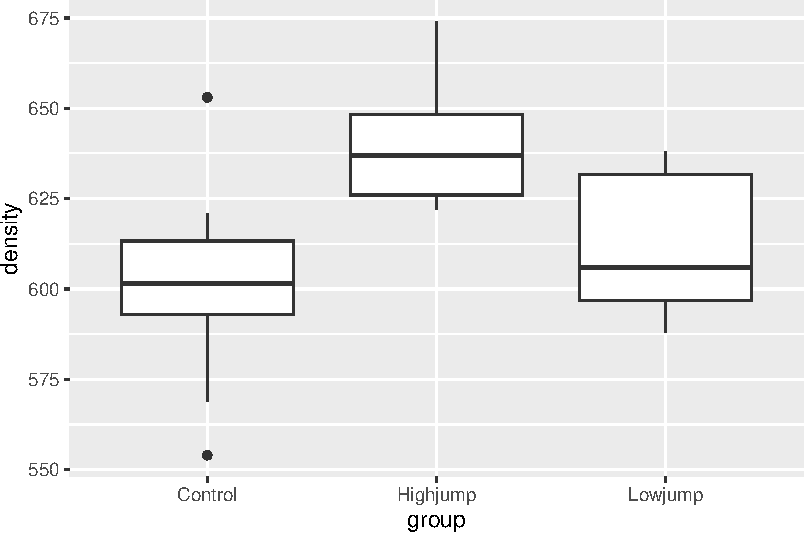
\includegraphics{inference_5_files/figure-pdf/inference-5-R-11-1.pdf}

}

\end{figure}

\hypertarget{or-arranging-groups-in-data-logical-order}{%
\subsection{Or, arranging groups in data (logical)
order}\label{or-arranging-groups-in-data-logical-order}}

\begin{Shaded}
\begin{Highlighting}[]
\FunctionTok{ggplot}\NormalTok{(rats, }\FunctionTok{aes}\NormalTok{(}\AttributeTok{y=}\NormalTok{density, }\AttributeTok{x=}\FunctionTok{fct\_inorder}\NormalTok{(group))) }\SpecialCharTok{+}
  \FunctionTok{geom\_boxplot}\NormalTok{()}
\end{Highlighting}
\end{Shaded}

\begin{figure}[H]

{\centering 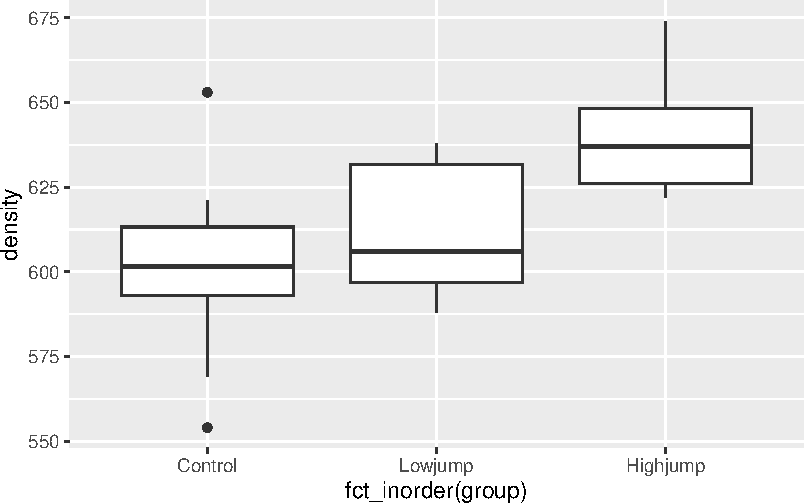
\includegraphics{inference_5_files/figure-pdf/inference-5-R-12-1.pdf}

}

\end{figure}

\hypertarget{analysis-of-variance}{%
\subsection{Analysis of Variance}\label{analysis-of-variance}}

\begin{itemize}
\tightlist
\item
  Comparing \textgreater{} 2 groups of independent observations (each
  rat only does one amount of jumping).
\item
  Standard procedure: analysis of variance (ANOVA).
\item
  Null hypothesis: all groups have same mean.
\item
  Alternative: ``not all means the same'', at least one is different
  from others.
\end{itemize}

\hypertarget{testing-anova-in-r}{%
\subsection{Testing: ANOVA in R}\label{testing-anova-in-r}}

\begin{Shaded}
\begin{Highlighting}[]
\NormalTok{rats.aov }\OtherTok{\textless{}{-}} \FunctionTok{aov}\NormalTok{(density}\SpecialCharTok{\textasciitilde{}}\NormalTok{group,}\AttributeTok{data=}\NormalTok{rats)}
\FunctionTok{summary}\NormalTok{(rats.aov)}
\end{Highlighting}
\end{Shaded}

\begin{verbatim}
            Df Sum Sq Mean Sq F value Pr(>F)   
group        2   7434    3717   7.978 0.0019 **
Residuals   27  12579     466                  
---
Signif. codes:  0 '***' 0.001 '**' 0.01 '*' 0.05 '.' 0.1 ' ' 1
\end{verbatim}

\begin{itemize}
\tightlist
\item
  Usual ANOVA table, small P-value: significant result.
\item
  Conclude that the mean bone densities are not all equal.
\item
  Reject null, but not very useful finding.
\end{itemize}

\hypertarget{which-groups-are-different-from-which}{%
\subsection{Which groups are different from
which?}\label{which-groups-are-different-from-which}}

\begin{itemize}
\tightlist
\item
  ANOVA really only answers half our questions: it says ``there are
  differences'', but doesn't tell us which groups different.
\item
  One possibility (not the best): compare all possible pairs of groups,
  via two-sample t.
\item
  First pick out each group:
\end{itemize}

\begin{Shaded}
\begin{Highlighting}[]
\NormalTok{rats }\SpecialCharTok{\%\textgreater{}\%} \FunctionTok{filter}\NormalTok{(group}\SpecialCharTok{==}\StringTok{"Control"}\NormalTok{) }\OtherTok{{-}\textgreater{}}\NormalTok{ controls}
\NormalTok{rats }\SpecialCharTok{\%\textgreater{}\%} \FunctionTok{filter}\NormalTok{(group}\SpecialCharTok{==}\StringTok{"Lowjump"}\NormalTok{) }\OtherTok{{-}\textgreater{}}\NormalTok{ lows}
\NormalTok{rats }\SpecialCharTok{\%\textgreater{}\%} \FunctionTok{filter}\NormalTok{(group}\SpecialCharTok{==}\StringTok{"Highjump"}\NormalTok{) }\OtherTok{{-}\textgreater{}}\NormalTok{ highs}
\end{Highlighting}
\end{Shaded}

\hypertarget{control-vs.-low}{%
\subsection{Control vs.~low}\label{control-vs.-low}}

\begin{Shaded}
\begin{Highlighting}[]
\FunctionTok{t.test}\NormalTok{(controls}\SpecialCharTok{$}\NormalTok{density, lows}\SpecialCharTok{$}\NormalTok{density)}
\end{Highlighting}
\end{Shaded}

\begin{verbatim}

    Welch Two Sample t-test

data:  controls$density and lows$density
t = -1.0761, df = 16.191, p-value = 0.2977
alternative hypothesis: true difference in means is not equal to 0
95 percent confidence interval:
 -33.83725  11.03725
sample estimates:
mean of x mean of y 
    601.1     612.5 
\end{verbatim}

No sig. difference here.

\hypertarget{control-vs.-high}{%
\subsection{Control vs.~high}\label{control-vs.-high}}

\begin{Shaded}
\begin{Highlighting}[]
\FunctionTok{t.test}\NormalTok{(controls}\SpecialCharTok{$}\NormalTok{density, highs}\SpecialCharTok{$}\NormalTok{density)}
\end{Highlighting}
\end{Shaded}

\begin{verbatim}

    Welch Two Sample t-test

data:  controls$density and highs$density
t = -3.7155, df = 14.831, p-value = 0.002109
alternative hypothesis: true difference in means is not equal to 0
95 percent confidence interval:
 -59.19139 -16.00861
sample estimates:
mean of x mean of y 
    601.1     638.7 
\end{verbatim}

These are different.

\hypertarget{low-vs.-high}{%
\subsection{Low vs.~high}\label{low-vs.-high}}

\begin{Shaded}
\begin{Highlighting}[]
\FunctionTok{t.test}\NormalTok{(lows}\SpecialCharTok{$}\NormalTok{density, highs}\SpecialCharTok{$}\NormalTok{density)}
\end{Highlighting}
\end{Shaded}

\begin{verbatim}

    Welch Two Sample t-test

data:  lows$density and highs$density
t = -3.2523, df = 17.597, p-value = 0.004525
alternative hypothesis: true difference in means is not equal to 0
95 percent confidence interval:
 -43.15242  -9.24758
sample estimates:
mean of x mean of y 
    612.5     638.7 
\end{verbatim}

These are different too.

\hypertarget{but}{%
\subsection{But\ldots{}}\label{but}}

\begin{itemize}
\tightlist
\item
  We just did 3 tests instead of 1.
\item
  So we have given ourselves 3 chances to reject \(H_0:\) all means
  equal, instead of 1.
\item
  Thus \(\alpha\) for this combined test is not 0.05.
\end{itemize}

\hypertarget{john-w.-tukey}{%
\subsection{John W. Tukey}\label{john-w.-tukey}}

\begin{columns}
    \begin{column}{0.4\textwidth}
      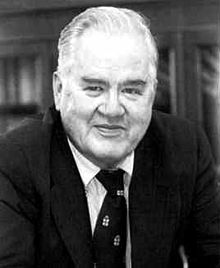
\includegraphics[width=\textwidth]{John_Tukey}
    \end{column}
    \begin{column}{0.6\textwidth}
      \begin{itemize}
      \item American statistician, 1915--2000
      \item Big fan of exploratory data analysis
      \item Invented boxplot
      \item Invented "honestly significant differences"
      \item Invented jackknife estimation
      \item Coined computing term "bit"
      \item Co-inventor of Fast Fourier Transform
      \end{itemize}
    \end{column}
  \end{columns}

\hypertarget{honestly-significant-differences}{%
\subsection{Honestly Significant
Differences}\label{honestly-significant-differences}}

\begin{itemize}
\tightlist
\item
  Compare several groups with one test, telling you which groups differ
  from which.
\item
  Idea: if all population means equal, find distribution of highest
  sample mean minus lowest sample mean.
\item
  Any means unusually different compared to that declared significantly
  different.
\end{itemize}

\hypertarget{tukey-on-rat-data}{%
\subsection{Tukey on rat data}\label{tukey-on-rat-data}}

\small

\begin{Shaded}
\begin{Highlighting}[]
\NormalTok{rats.aov }\OtherTok{\textless{}{-}} \FunctionTok{aov}\NormalTok{(density}\SpecialCharTok{\textasciitilde{}}\NormalTok{group, }\AttributeTok{data =}\NormalTok{ rats)}
\FunctionTok{TukeyHSD}\NormalTok{(rats.aov)}
\end{Highlighting}
\end{Shaded}

\begin{verbatim}
  Tukey multiple comparisons of means
    95% family-wise confidence level

Fit: aov(formula = density ~ group, data = rats)

$group
                  diff       lwr       upr     p adj
Highjump-Control  37.6  13.66604 61.533957 0.0016388
Lowjump-Control   11.4 -12.53396 35.333957 0.4744032
Lowjump-Highjump -26.2 -50.13396 -2.266043 0.0297843
\end{verbatim}

\normalsize

\begin{itemize}
\tightlist
\item
  Again conclude that bone density for highjump group significantly
  higher than for other two groups.
\end{itemize}

\hypertarget{why-tukeys-procedure-better-than-all-t-tests}{%
\subsection{Why Tukey's procedure better than all
t-tests}\label{why-tukeys-procedure-better-than-all-t-tests}}

Look at P-values for the two tests:

\begin{verbatim}
Comparison        Tukey    t-tests
----------------------------------
Highjump-Control 0.0016     0.0021
Lowjump-Control  0.4744     0.2977
Lowjump-Highjump 0.0298     0.0045
\end{verbatim}

\begin{itemize}
\tightlist
\item
  Tukey P-values (mostly) higher.
\item
  Proper adjustment for doing three t-tests at once, not just one in
  isolation.
\end{itemize}

\hypertarget{checking-assumptions}{%
\subsection{Checking assumptions}\label{checking-assumptions}}

\begin{Shaded}
\begin{Highlighting}[]
\FunctionTok{ggplot}\NormalTok{(rats,}\FunctionTok{aes}\NormalTok{(}\AttributeTok{y =}\NormalTok{ density, }\AttributeTok{x =} \FunctionTok{fct\_inorder}\NormalTok{(group)))}\SpecialCharTok{+}
  \FunctionTok{geom\_boxplot}\NormalTok{()}
\end{Highlighting}
\end{Shaded}

\begin{figure}[H]

{\centering 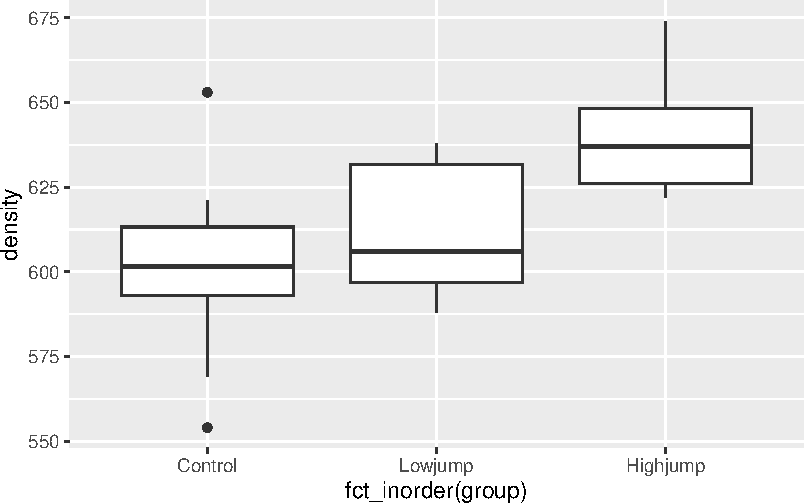
\includegraphics{inference_5_files/figure-pdf/inference-5-R-21-1.pdf}

}

\end{figure}

Assumptions:

\begin{itemize}
\tightlist
\item
  Normally distributed data within each group
\item
  with equal group SDs.
\end{itemize}

\hypertarget{normal-quantile-plots-by-group}{%
\subsection{Normal quantile plots by
group}\label{normal-quantile-plots-by-group}}

\begin{Shaded}
\begin{Highlighting}[]
\FunctionTok{ggplot}\NormalTok{(rats, }\FunctionTok{aes}\NormalTok{(}\AttributeTok{sample =}\NormalTok{ density)) }\SpecialCharTok{+} \FunctionTok{stat\_qq}\NormalTok{() }\SpecialCharTok{+} 
  \FunctionTok{stat\_qq\_line}\NormalTok{() }\SpecialCharTok{+} \FunctionTok{facet\_wrap}\NormalTok{( }\SpecialCharTok{\textasciitilde{}}\NormalTok{ group)}
\end{Highlighting}
\end{Shaded}

\begin{figure}[H]

{\centering 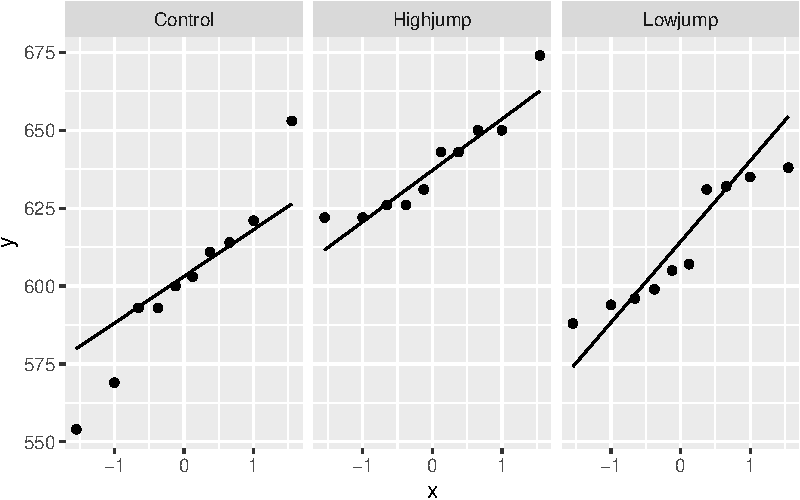
\includegraphics{inference_5_files/figure-pdf/inference-5-R-22-1.pdf}

}

\end{figure}

\hypertarget{the-assumptions}{%
\subsection{The assumptions}\label{the-assumptions}}

\begin{itemize}
\tightlist
\item
  Normally-distributed data within each group
\item
  Equal group SDs.
\item
  These are shaky here because:

  \begin{itemize}
  \tightlist
  \item
    control group has outliers
  \item
    highjump group appears to have less spread than others.
  \end{itemize}
\item
  Possible remedies (in general):

  \begin{itemize}
  \tightlist
  \item
    Transformation of response (usually works best when SD increases
    with mean)
  \item
    If normality OK but equal spreads not, can use Welch ANOVA. (Regular
    ANOVA like pooled t-test; Welch ANOVA like Welch-Satterthwaite
    t-test.)
  \item
    Can also use Mood's Median Test (see over). This works for any
    number of groups.
  \end{itemize}
\end{itemize}

\hypertarget{moods-median-test-14}{%
\subsection{Mood's median test 1/4}\label{moods-median-test-14}}

\begin{itemize}
\tightlist
\item
  Find median of all bone densities, regardless of group:
\end{itemize}

\small

\begin{Shaded}
\begin{Highlighting}[]
\NormalTok{(rats }\SpecialCharTok{\%\textgreater{}\%} \FunctionTok{summarize}\NormalTok{(}\AttributeTok{med =} \FunctionTok{median}\NormalTok{(density)) }\SpecialCharTok{\%\textgreater{}\%} \FunctionTok{pull}\NormalTok{(med) }\OtherTok{{-}\textgreater{}}\NormalTok{ m)}
\end{Highlighting}
\end{Shaded}

\begin{verbatim}
[1] 621.5
\end{verbatim}

\normalsize

\begin{itemize}
\tightlist
\item
  Count up how many observations in each group above or below overall
  median:
\end{itemize}

\begin{Shaded}
\begin{Highlighting}[]
\NormalTok{tab }\OtherTok{\textless{}{-}} \FunctionTok{with}\NormalTok{(rats, }\FunctionTok{table}\NormalTok{(group, density }\SpecialCharTok{\textgreater{}}\NormalTok{ m))}
\NormalTok{tab}
\end{Highlighting}
\end{Shaded}

\begin{verbatim}
          
group      FALSE TRUE
  Control      9    1
  Highjump     0   10
  Lowjump      6    4
\end{verbatim}

\hypertarget{moods-median-test-24}{%
\subsection{Mood's median test 2/4}\label{moods-median-test-24}}

\begin{Shaded}
\begin{Highlighting}[]
\NormalTok{tab}
\end{Highlighting}
\end{Shaded}

\begin{verbatim}
          
group      FALSE TRUE
  Control      9    1
  Highjump     0   10
  Lowjump      6    4
\end{verbatim}

\begin{itemize}
\tightlist
\item
  All Highjump obs above overall median.
\item
  Most Control obs below overall median.
\item
  Suggests medians differ by group.
\end{itemize}

\hypertarget{moods-median-test-34}{%
\subsection{Mood's median test 3/4}\label{moods-median-test-34}}

\begin{itemize}
\tightlist
\item
  Test whether association between group and being above/below overall
  median significant using chi-squared test for association:
\end{itemize}

\begin{Shaded}
\begin{Highlighting}[]
\FunctionTok{chisq.test}\NormalTok{(tab,}\AttributeTok{correct=}\NormalTok{F)}
\end{Highlighting}
\end{Shaded}

\begin{verbatim}

    Pearson's Chi-squared test

data:  tab
X-squared = 16.8, df = 2, p-value = 0.0002249
\end{verbatim}

\begin{itemize}
\tightlist
\item
  Very small P-value says that being above/below overall median depends
  on group.
\item
  That is, groups do not all have same median.
\end{itemize}

\hypertarget{moods-median-test-44}{%
\subsection{Mood's median test 4/4}\label{moods-median-test-44}}

Or with \texttt{median\_test} from \texttt{smmr}, same as before.

\begin{Shaded}
\begin{Highlighting}[]
\FunctionTok{median\_test}\NormalTok{(rats,density,group)}
\end{Highlighting}
\end{Shaded}

\begin{verbatim}
$table
          above
group      above below
  Control      1     9
  Highjump    10     0
  Lowjump      4     6

$test
       what        value
1 statistic 1.680000e+01
2        df 2.000000e+00
3   P-value 2.248673e-04
\end{verbatim}

\hypertarget{comments}{%
\subsection{Comments}\label{comments}}

\begin{itemize}
\tightlist
\item
  No doubt that medians differ between groups (not all same).
\item
  This test is equivalent of \(F\)-test, not of Tukey.
\item
  To determine which groups differ from which, can compare all possible
  pairs of groups via (2-sample) Mood's median tests, then adjust
  P-values by multiplying by number of 2-sample Mood tests done
  (Bonferroni):
\end{itemize}

\begin{Shaded}
\begin{Highlighting}[]
\FunctionTok{pairwise\_median\_test}\NormalTok{(rats,density,group)}
\end{Highlighting}
\end{Shaded}

\begin{verbatim}
# A tibble: 3 x 4
  g1       g2        p_value adj_p_value
  <chr>    <chr>       <dbl>       <dbl>
1 Control  Highjump 0.000148    0.000443
2 Control  Lowjump  0.371       1       
3 Highjump Lowjump  0.371       1       
\end{verbatim}

\begin{itemize}
\tightlist
\item
  Now, lowjump-highjump difference no longer significant.
\end{itemize}

\hypertarget{welch-anova}{%
\subsection{Welch ANOVA}\label{welch-anova}}

\begin{itemize}
\tightlist
\item
  For these data, Mood's median test probably best because we doubt both
  normality and equal spreads.
\item
  When normality OK but spreads differ, Welch ANOVA way to go.
\item
  Welch ANOVA done by \texttt{oneway.test} as shown (for illustration):
\end{itemize}

\begin{Shaded}
\begin{Highlighting}[]
\FunctionTok{oneway.test}\NormalTok{(density}\SpecialCharTok{\textasciitilde{}}\NormalTok{group,}\AttributeTok{data=}\NormalTok{rats)}
\end{Highlighting}
\end{Shaded}

\begin{verbatim}

    One-way analysis of means (not assuming equal variances)

data:  density and group
F = 8.8164, num df = 2.000, denom df = 17.405, p-value = 0.002268
\end{verbatim}

\begin{itemize}
\tightlist
\item
  P-value very similar, as expected.
\item
  Appropriate Tukey-equivalent here called Games-Howell.
\end{itemize}

\hypertarget{games-howell}{%
\subsection{Games-Howell}\label{games-howell}}

\begin{itemize}
\tightlist
\item
  Lives in package \texttt{PMCMRplus}. Install first.
\end{itemize}

\begin{Shaded}
\begin{Highlighting}[]
\FunctionTok{library}\NormalTok{(PMCMRplus)}
\end{Highlighting}
\end{Shaded}

\begin{Shaded}
\begin{Highlighting}[]
\FunctionTok{gamesHowellTest}\NormalTok{(density}\SpecialCharTok{\textasciitilde{}}\FunctionTok{factor}\NormalTok{(group),}\AttributeTok{data=}\NormalTok{rats)}
\end{Highlighting}
\end{Shaded}

\begin{verbatim}

    Pairwise comparisons using Games-Howell test
\end{verbatim}

\begin{verbatim}
data: density by factor(group)
\end{verbatim}

\begin{verbatim}
         Control Highjump
Highjump 0.0056  -       
Lowjump  0.5417  0.0120  
\end{verbatim}

\begin{verbatim}

P value adjustment method: none
\end{verbatim}

\begin{verbatim}
alternative hypothesis: two.sided
\end{verbatim}

\hypertarget{deciding-which-test-to-do}{%
\subsection{Deciding which test to do}\label{deciding-which-test-to-do}}

For two or more samples:

\begin{figure}

{\centering 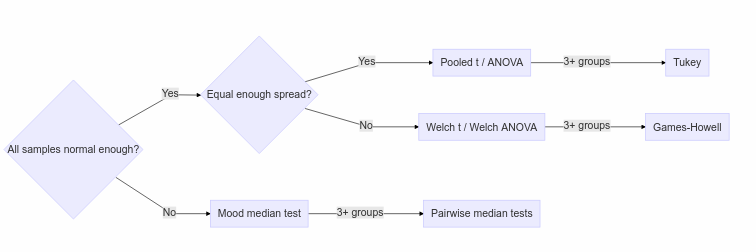
\includegraphics{testflow.png}

}

\caption{Test flow chart}

\end{figure}



\end{document}
